%% Assignment #3 for B-trees and Binomial Heaps

\documentclass[10pt,fullpage]{article}

\usepackage{amsmath,amssymb,amsthm,amsfonts} % Typical maths resource packages

%Check if we are compiling under latex or pdflatex
\ifx\pdftexversion\undefined
\usepackage[dvips]{graphicx}
%%%%%%%%
%% Pour inclure du .jpg et .pnm sous latex
%%%%%%%%%%%%%%
\DeclareGraphicsExtensions{.jpg,.eps,.pnm}
\DeclareGraphicsRule{.jpg}{eps}{.jpg.bb}{`jpeg2ps -h #1}
\DeclareGraphicsRule{.pnm}{eps}{.pnm.bb}{`pnmtops #1} \else
\usepackage[pdftex]{graphicx}
\fi

\usepackage{hyperref}                 % For creating hyperlinks in cross references

\usepackage{listings}

\usepackage{qtree}

\topmargin -1.5cm \oddsidemargin -0.04cm \evensidemargin -0.04cm
\textwidth 16.00cm \textheight 23.50cm
\parskip 7.2pt
\parindent 0.25in

\makeindex

\title{ Advanced Algorithms Assignment III }


\author{Matthew Bennett \\
{\small\em B-Trees and Binomial Heaps HW \ Draft date \today }}

 \date{ }

\begin{document}
\maketitle

\textbf{Exercises 18.2-1 Show the results of inserting the keys F,
S, Q, K, C, L, H, T, V, W, M, R, N, P, A, B, X, Y, D, Z, E in
order into an empty B-tree with minimum degree 3. Only draw the
configurations of the tree just before some node must split, and
also draw the final configuration.
}\\

\Tree [.{C F K Q S} ]

\Tree [.K [.{C F} ] [.{Q S} ] ]

\Tree [.K [.{C F H} ] [.{L Q S T V} ] ]

\Tree [.{K S} [.{C F H} ] [.{L Q} ] [.{T V} ] ]

\Tree [.{K S} [.{C F H} ] [.{L M N Q R} ] [.{T V W} ] ]

\Tree [.{K N S} [.{C F H} ] [.{L M} ] [.{Q R} ] [.{T V W} ] ]

\Tree [.{K N S} [.{A B C F H} ] [.{L M} ] [.{P Q R} ] [.{T V W X Y}
] ]

\Tree [.{C K N S} [.{A B} ] [.{D F H} ] [.{L M} ] [.{P Q R} ] [.{T V
W X Y} ] ]

\Tree [.{C K N S W} [.{A B} ] [.{D F H} ] [.{L M} ] [.{P Q R} ] [.{T
V} ] [.{X Y Z} ] ]

(Step skipped intentionally due to \LaTeX restrictions)

\begin{figure}[h]\caption{Final Result}
\Tree [.N [.{C K} [.{A B} ] [.{D E F H} ] [.{L M} ] ] [.{S W} [.{P Q
R} ] [.{T V} ] [.{X Y Z} ] ] ]
\end{figure}
\newpage
\textbf{Exercises 18.2-3 Explain how to find the minimum key
stored in a B-tree and how to find the predecessor of a given key
stored in a B-tree.}\\

To find the minimum key, use the following method: starting at the
root, if the current node is a leaf, return the leftmost element.
Otherwise, recurse into the leftmost child pointer.\\
To find the predecessor of a key, start at the node of that key.
\\\textbf{CASE 1: If there is a child node between the previous key in
that node (or null) and the key.} Visit it and return the rightmost
key if that node is a leaf. Otherwise, visit the rightmost child
node and recurse.
\\\textbf{CASE 2: If the key is the leftmost member of a node with no children left of the key.} Visit its
parent. The last member of member of that node which precedes the
key will be the predecessor.
\\\textbf{CASE 3: If the key is the only member of a root node with no children.}
Then its predecessor does not exist. Return null.

\newpage

\textbf{Exercises 19.1-1 Suppose that x is a node in a binomial tree
within a binomial heap, and assume that sibling[x] $\neq$ NIL. If x
is not a root, how does degree[sibling[x]] compare to degree[x]? How
about if x is a root? }

Assume x is the root of a subtree $B_k$ with degree $k$ and x has a
sibling. If x is not a root then the sibling must be root of a the
next subtree, $B_{k-1}$, by the binomial heap definition.\\
If x is a root then the next tree occurring in the root list must be
the tree $B_i$, where $i$ is the position of the next 1-bit in
the binary representation of the number of nodes.\\

\textbf{Exercises 19.1-2 If x is a non-root node in a binomial tree
within a binomial heap, how does degree[x] compare to
degree[parent[x]]? }

$degree[parent[x]] = 1 + degree[x] $, since:
the root has degree $k$, which is greater than that of any other node; moreover if $i$ the children of the root are numbered from left to right by $k - 1, k - 2, \ldots, 0,$ child i is the root of a subtree $B_i$\\

\newpage

\textbf{Exercises 19.2-2 Show the binomial heap that results when a
node with key 24 is inserted into the binomial heap shown in Figure
19.7(d). }\\

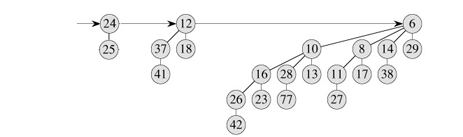
\includegraphics{fig1907D.png}

\textbf{Exercises 19.2-3 Show the binomial heap that results when
the node with key 28 is deleted from the binomial heap shown in
Figure 19.8(c). }\\

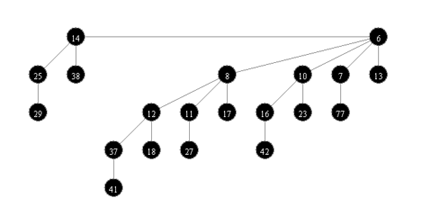
\includegraphics{fig1908C.png}

\newpage


\end{document}
